\documentclass{article}
\usepackage{tikz,amsmath,siunitx}
\usetikzlibrary{calc}
\usetikzlibrary{positioning}
\usetikzlibrary{arrows,snakes,backgrounds,patterns,matrix,shapes,fit,calc,shadows,plotmarks}
\usepackage[graphics,tightpage,active]{preview}
\PreviewEnvironment{tikzpicture}
\PreviewEnvironment{equation}
\PreviewEnvironment{equation*}
\newlength{\imagewidth}
\newlength{\imagescale}
\pagestyle{empty}
\thispagestyle{empty}
\begin{document}
  \begin{tikzpicture} [auto, node distance=0cm]
   \node at (0,0) (A) {
\begin{tikzpicture}
    \node [anchor=south west] at (0,0) (foo) {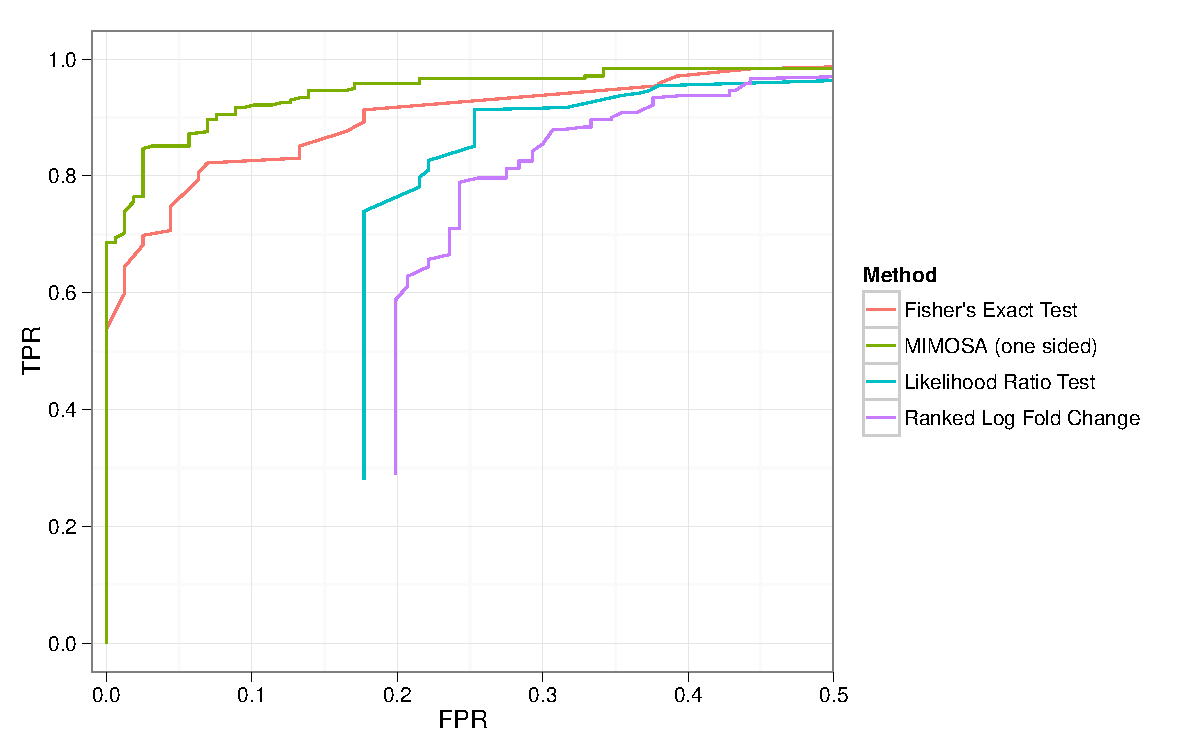
\includegraphics[width=0.5\columnwidth]{Figures/Sim_Onesided_ROC_5000.pdf}};
    \begin{scope}[x={(foo.south east)},y={(foo.north west)}]
        \node at (0,1) [font=\tiny\sffamily] {A} ;
        \end{scope}
    \end{tikzpicture}
    };
    \node [right=of A] (B) {
    \begin{tikzpicture}
    \node [anchor=south west] at (0,0) (bar) {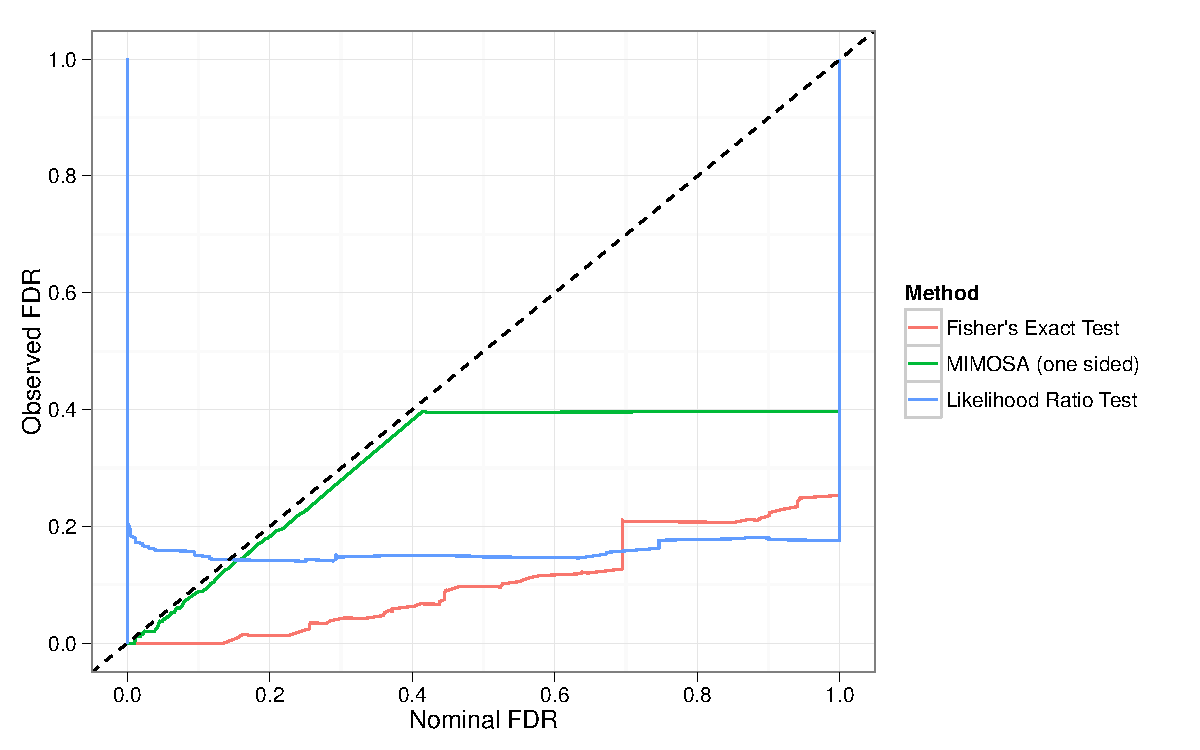
\includegraphics[width=0.5\columnwidth]{Figures/Sim_Onesided_FDR_5000.pdf}};
    \begin{scope}[x={(bar.south east)},y={(bar.north west)}]
    \node at (0,1) [font=\tiny\sffamily] {B} ;
    \end{scope}
    \end{tikzpicture}
    };
        \node [below=of A] (C) {
    \begin{tikzpicture}
    \node [anchor=south west] at (0,0) (c) {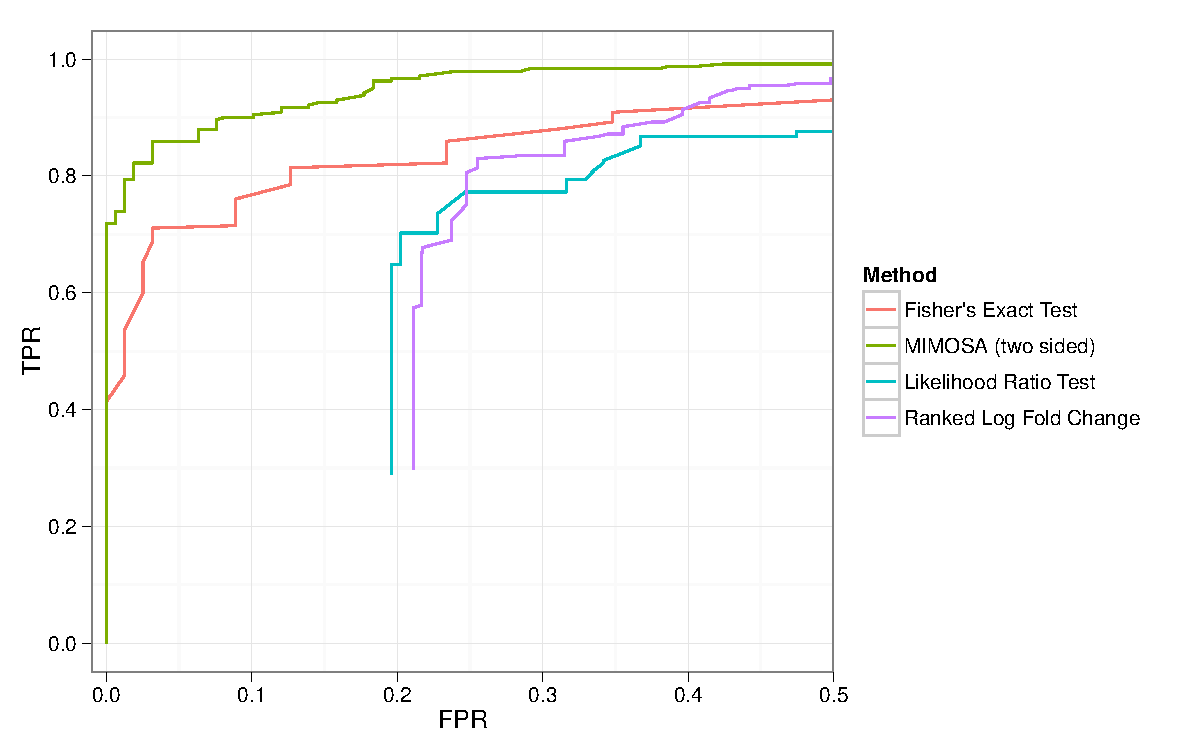
\includegraphics[width=0.5\columnwidth]{Figures/Sim_Twosided_ROC_5000.pdf}};
    \begin{scope}[x={(c.south east)},y={(c.north west)}]
    \node at (0,1) [font=\tiny\sffamily] {C} ;
    \end{scope}
    \end{tikzpicture}
    };
    \node [right=of C] (D) {
    \begin{tikzpicture}
    \node [anchor=south west] at (0,0) (d) {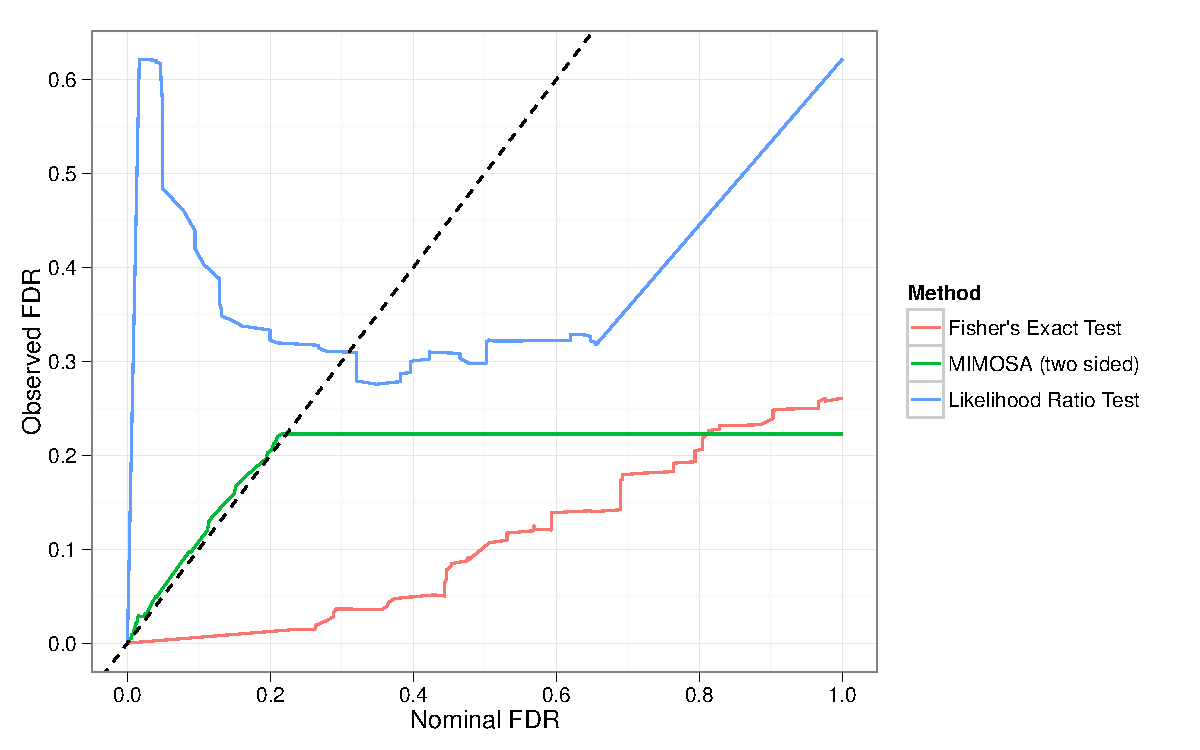
\includegraphics[width=0.5\columnwidth]{Figures/Sim_Twosided_FDR_5000.pdf}};
    \begin{scope}[x={(d.south east)},y={(d.north west)}]
    \node at (0,1) [font=\tiny\sffamily] {D} ;
    \end{scope}
    \end{tikzpicture}
    };

\end{tikzpicture}
\end{document}
